%!TEX program = xelatex
% Note: this template must be compiled with XeLaTeX rather than PDFLaTeX
% due to the custom fonts used. The line above should ensure this happens
% automatically, but if it doesn't, your LaTeX editor should have a simple toggle
% to switch to using XeLaTeX.

\documentclass[
  aspectratio=169, % Uncomment to use an aspect ratio of 16:9 (160 mm by 90 mm)
  %aspectratio=43, % Uncomment to use an aspect ratio of 4:3 (128mm by 96mm)
  t, % Top align all slide content by default
  onlytextwidth, % Typeset content in columns at text width
  10pt, % Default font size, use 10pt for the 16:9 aspect ratio and 8pt for the 4:3 aspect ratio
]{beamer}

\usepackage{../../ImperialTheme/beamer/beamerthemeImperial} % Use the Imperial theme

\def\imagefolder{../../ImperialTheme/beamer/Images}
\def\Rey{\text{Re}}
\title{Exploring more depths} % Presentation title to appear on the title slide and left footers

\subtitle{} % Presentation subtitle to appear on the title slide

\author{Víctor Ballester} % Author name(s) to appear on the title slide

\date{\today} % Presentation date to appear on the title slide and right footers

\begin{document}

\begingroup
\setbeamercolor{background canvas}{bg=ICLBlue} % Slide background color
\setbeamercolor{title page title}{fg=white} % Title text color
\setbeamercolor{title page subtitle}{fg=white} % Subtitle text color
\setbeamercolor{author}{fg=white} % Author(s) text color
\setbeamercolor{date}{fg=white} % Date text color
\setbeamertemplate{title page}[logo]{\imagefolder/ICL_Logo_White.pdf} % Imperial logo color, use 'ICL_Logo_White.pdf' for white and 'ICL_Logo_Blue.pdf' for blue
\frame[plain, s]{\titlepage} % Output the title page with no footer ('plain') and vertically distributed text ('s')
\endgroup

\begin{frame}
	\frametitle{General Comments}
	\begin{itemize}
		\item I confirm, we may still have a subcritical bifurcation in the vicinity of $d = 4\delta^*$, $w = 16\delta^*$. I ran a perturbed system in an unstable
		      configuration and I got a stable solution.
		\item Modified Arnoldi still doesn't output the TS mode for the stable case, now that the BC are (more) correct. We still get that huge mode. Should we go for blowing and suction?
		\item I ran a lot of runs varying $d/\delta^* \in [ 1,4 ]$ and $w/\delta^* \in [ 15, 130 ]$.
	\end{itemize}
\end{frame}
\begin{frame}
	\frametitle{Results}
	We know there's always a convectively unstable TS mode, even in the blue curve. My hypothesis (taken with caution) for the region $\{d/delta^*\leq 2.25\}$ is that if at some fixed $d$ we get an absolute unstable mode localized in the downstream edge of the gap, then as we increase $w$, the wavelength associated to the absolute mode becomes convectively unstable. 
	
	\centering
	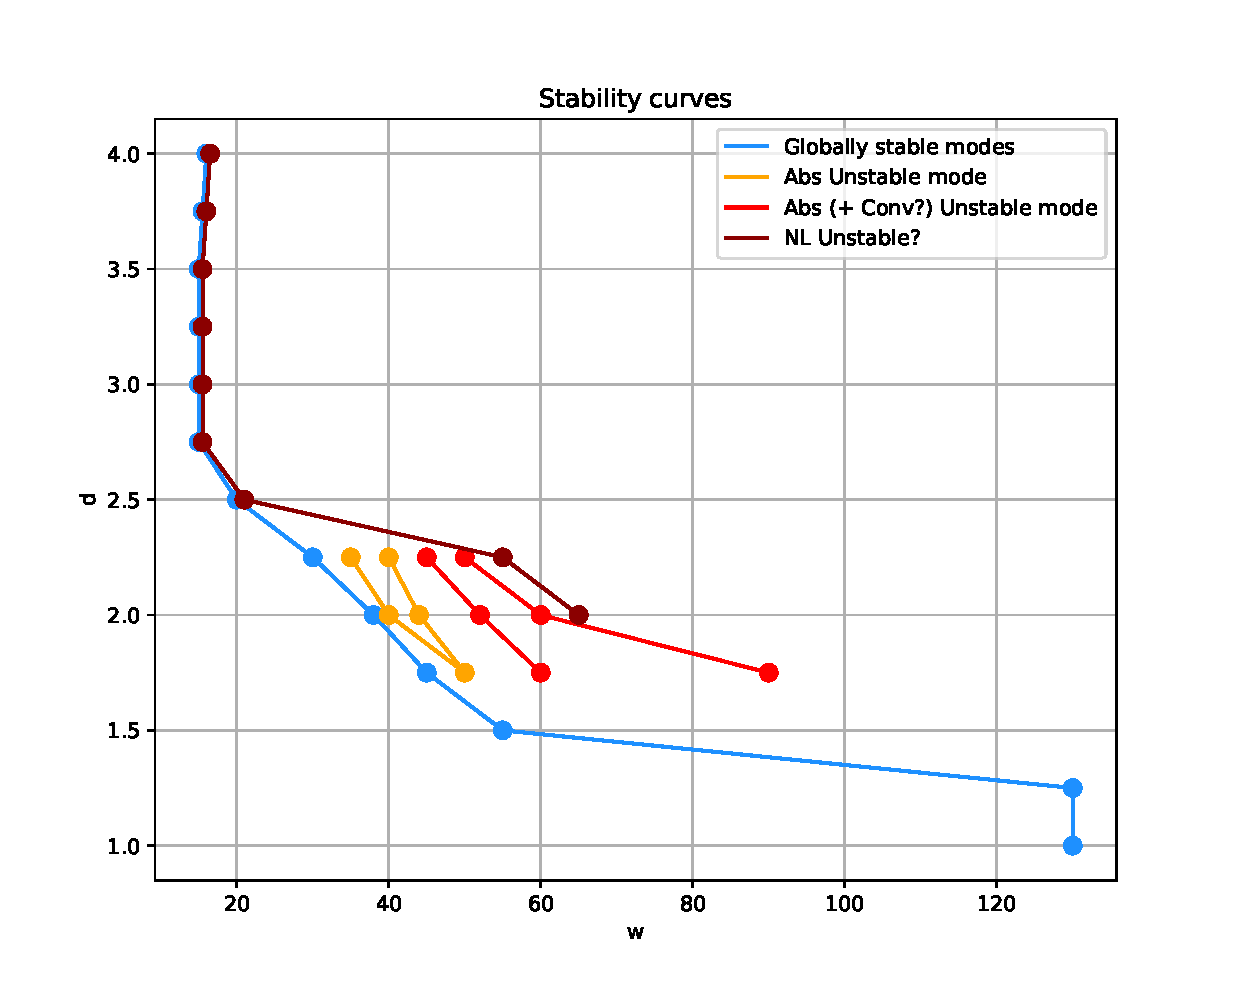
\includegraphics[width=0.5\linewidth]{Images/stabilitycurves.pdf}
\end{frame}
\begin{frame}
	\frametitle{$d=2.25\delta^*$}
	
	\centering
	\begin{columns}[T] % [T] ensures correct vertical alignment
		\begin{column}{0.45\linewidth} % Left column
			$w=35\delta^*$

			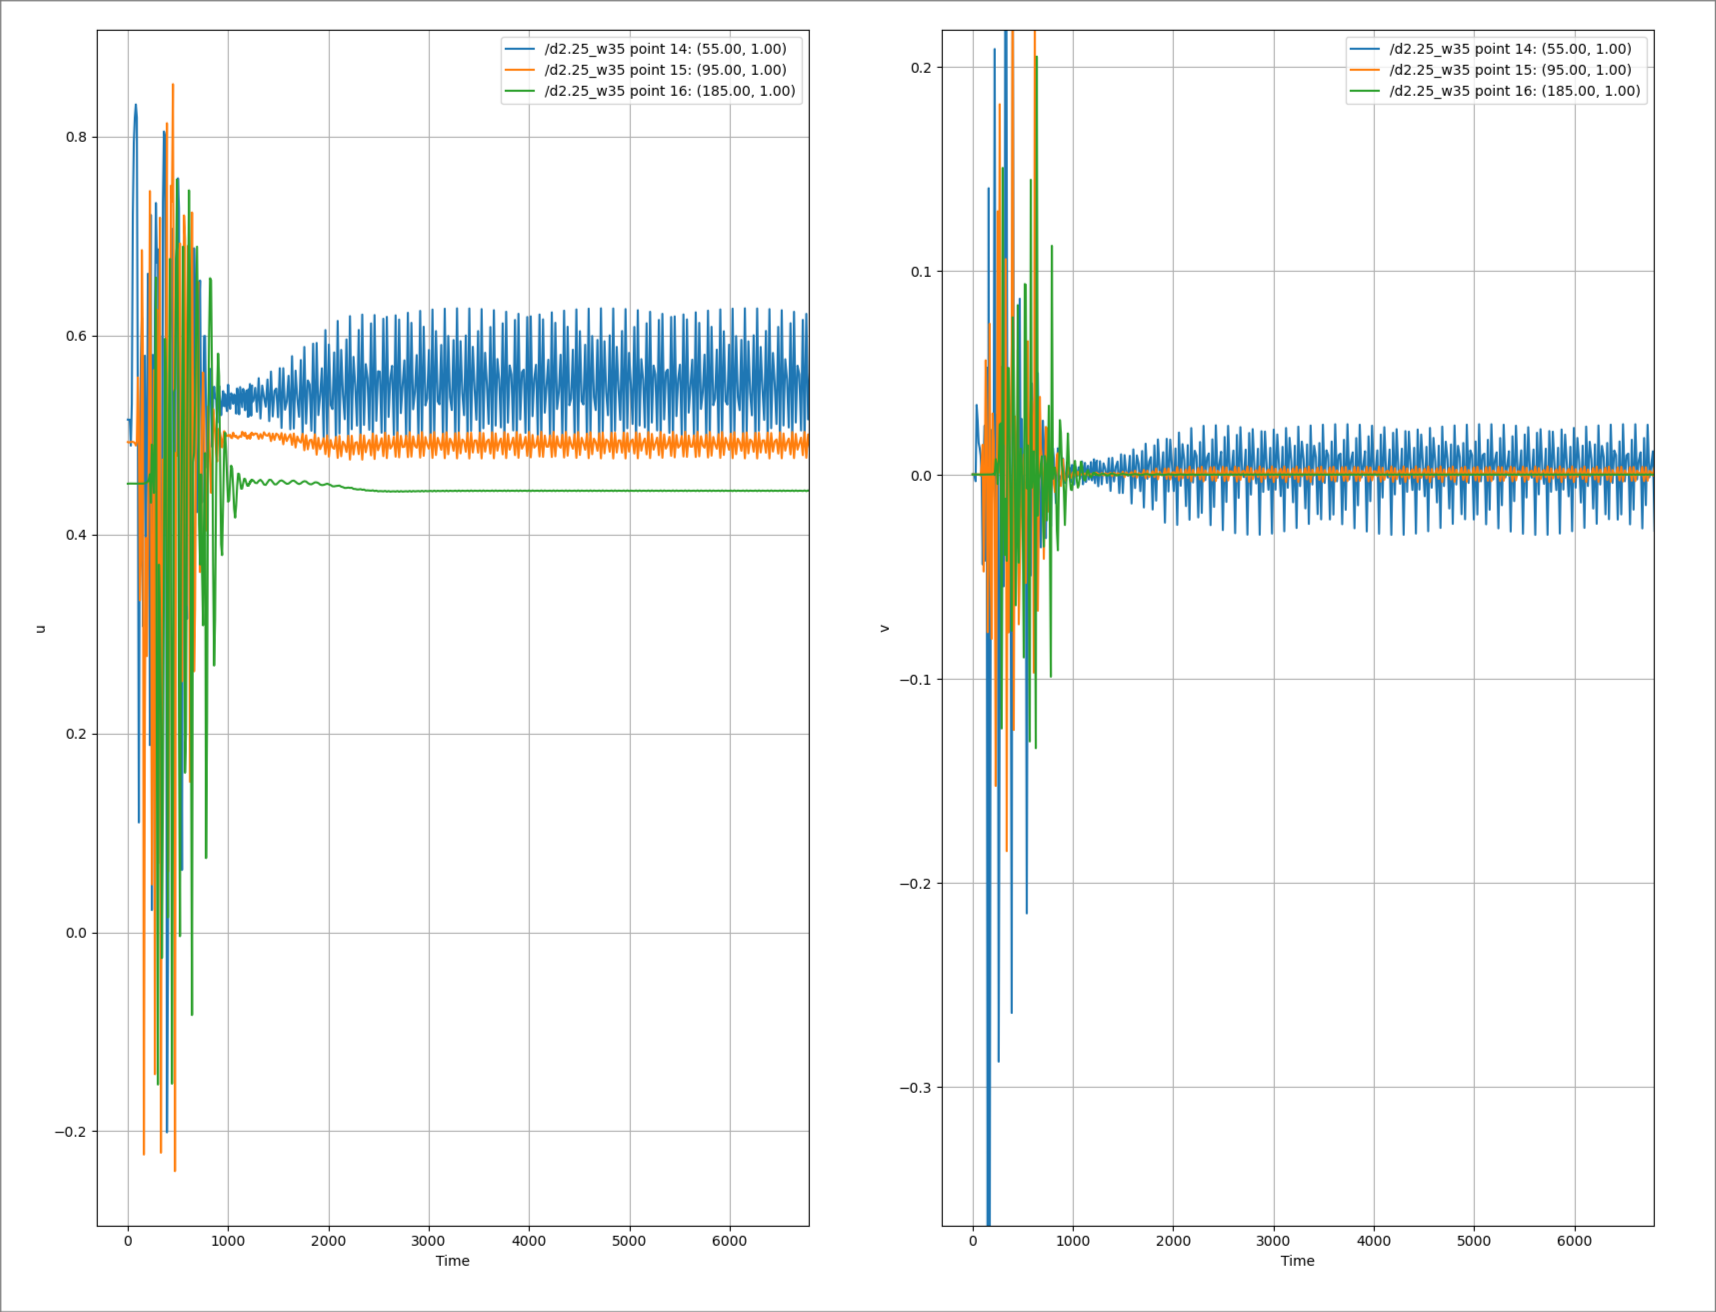
\includegraphics[width=\textwidth]{Images/d2.25_w35.png}
			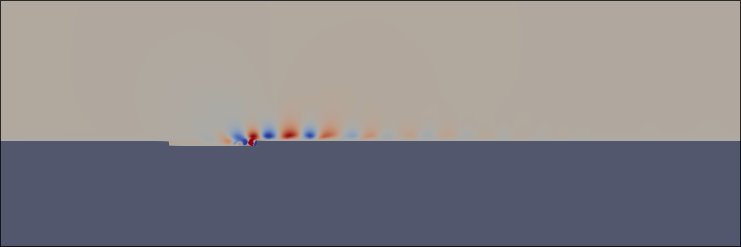
\includegraphics[width=\textwidth]{Images/d2.25_w35_dom.png}
		\end{column}
		\begin{column}{0.45\linewidth} % Left column
			$w=40\delta^*$	

			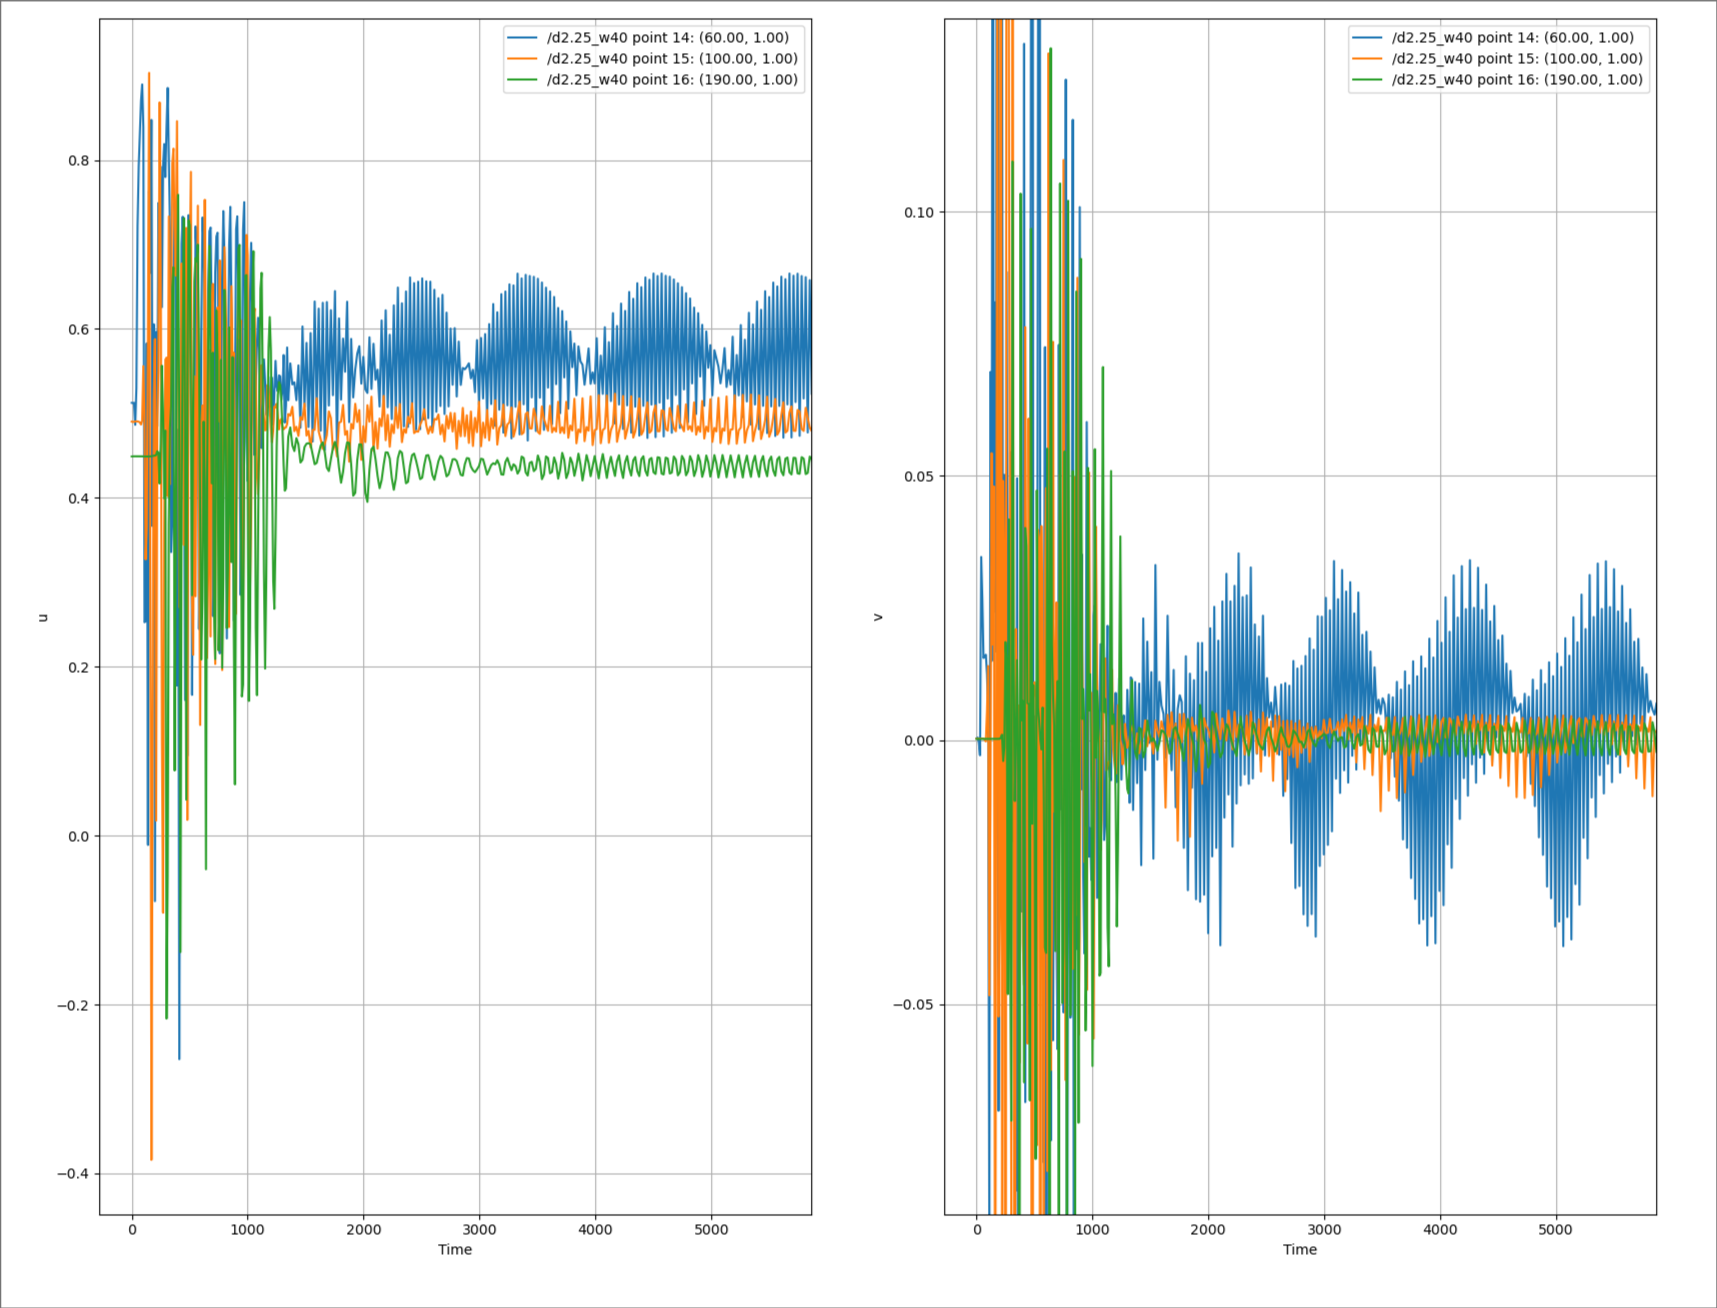
\includegraphics[width=\textwidth]{Images/d2.25_w40.png}
			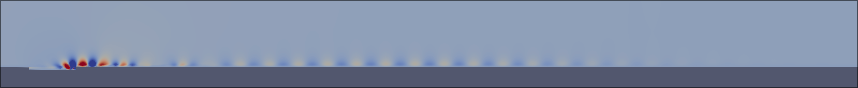
\includegraphics[width=\textwidth]{Images/d2.25_w40_dom.png}
		\end{column}
	\end{columns}
\end{frame}
\begin{frame}
	\frametitle{$d=2.25\delta^*$}
	
	\centering
	\begin{columns}[T] % [T] ensures correct vertical alignment
		\begin{column}{0.45\linewidth} % Left column
			$w=45\delta^*$

			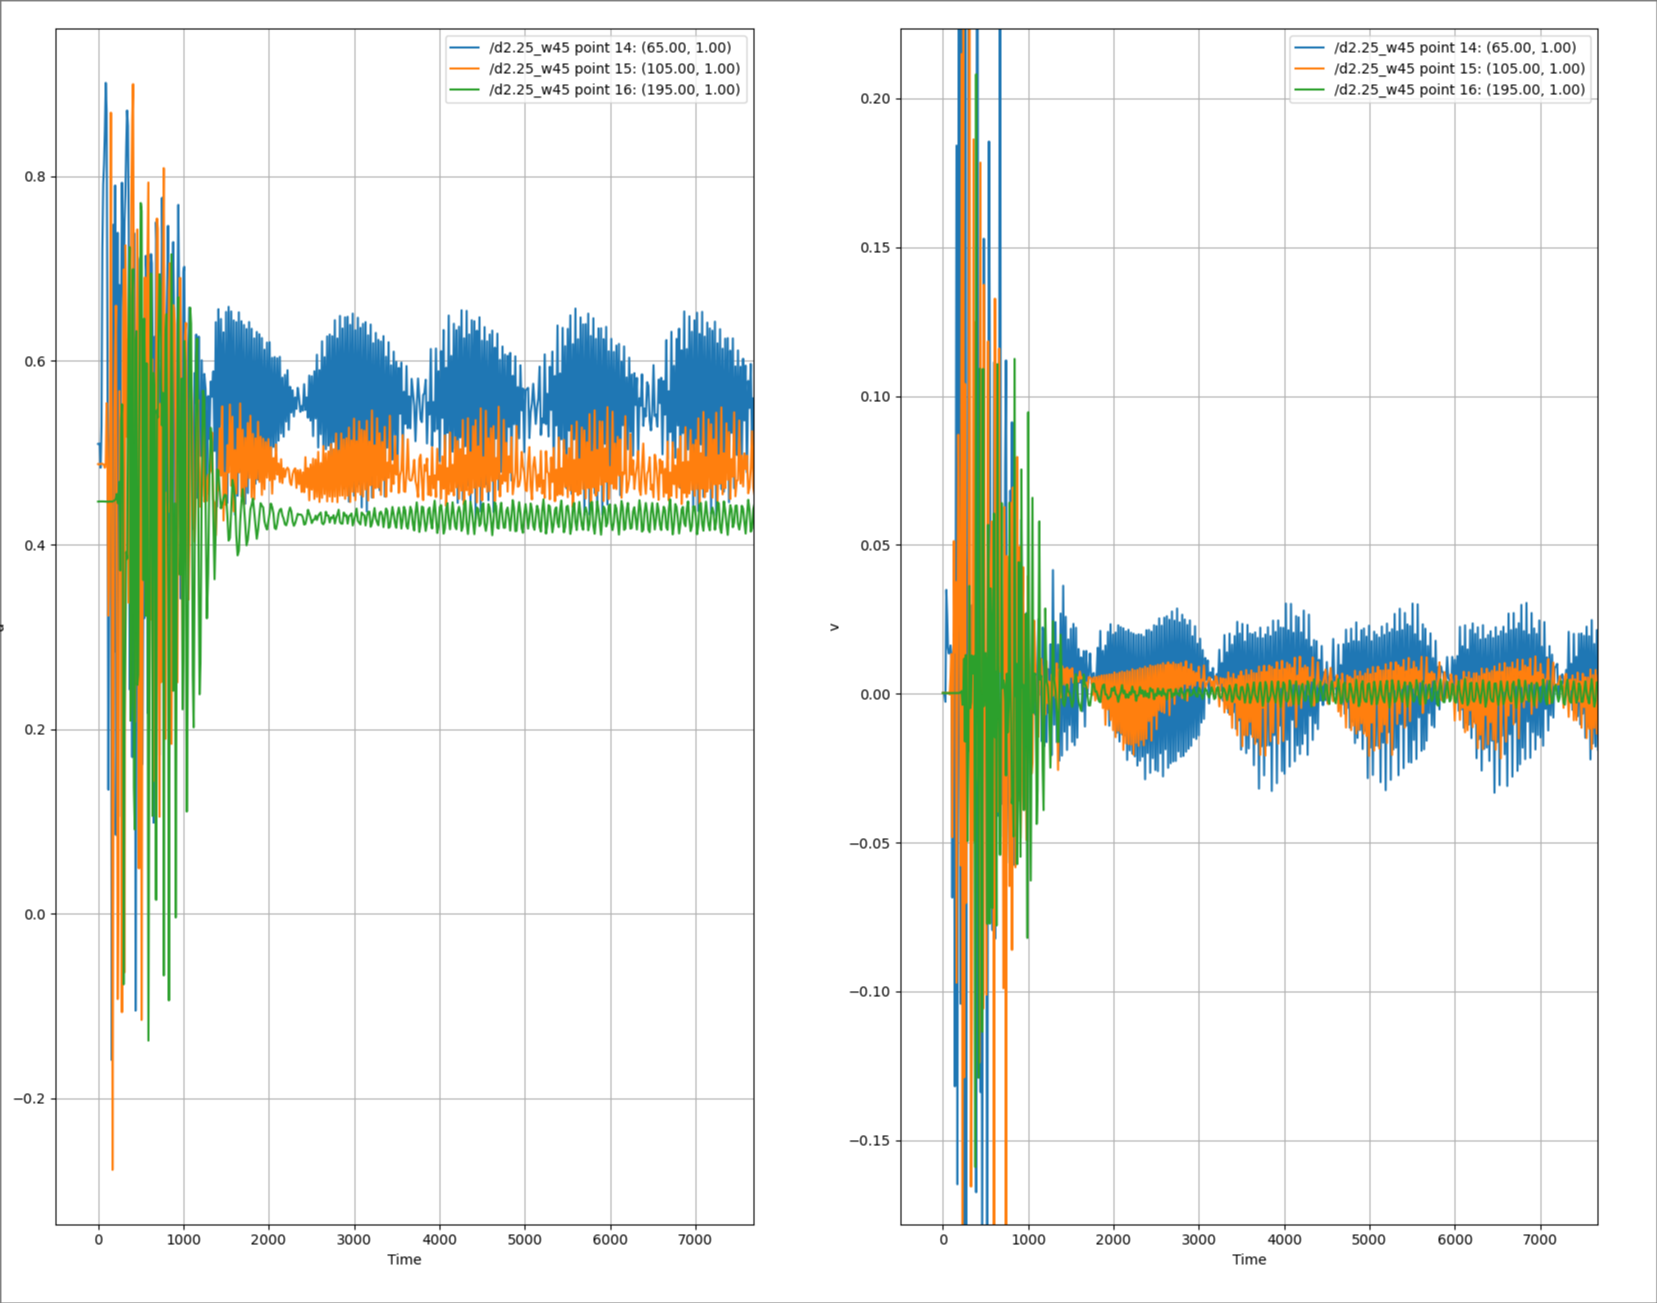
\includegraphics[width=\textwidth]{Images/d2.25_w45.png}
			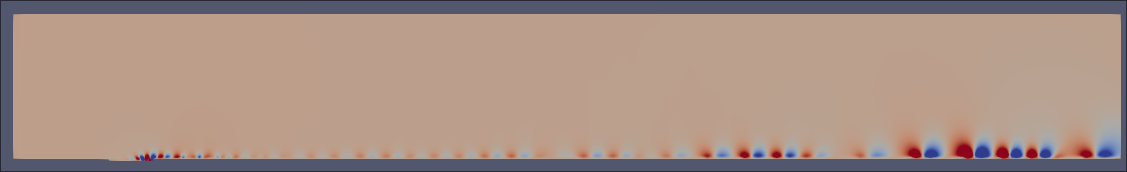
\includegraphics[width=\textwidth]{Images/d2.25_w45_dom.png}
		\end{column}
		\begin{column}{0.45\linewidth} % Left column
			$w=50\delta^*$	

			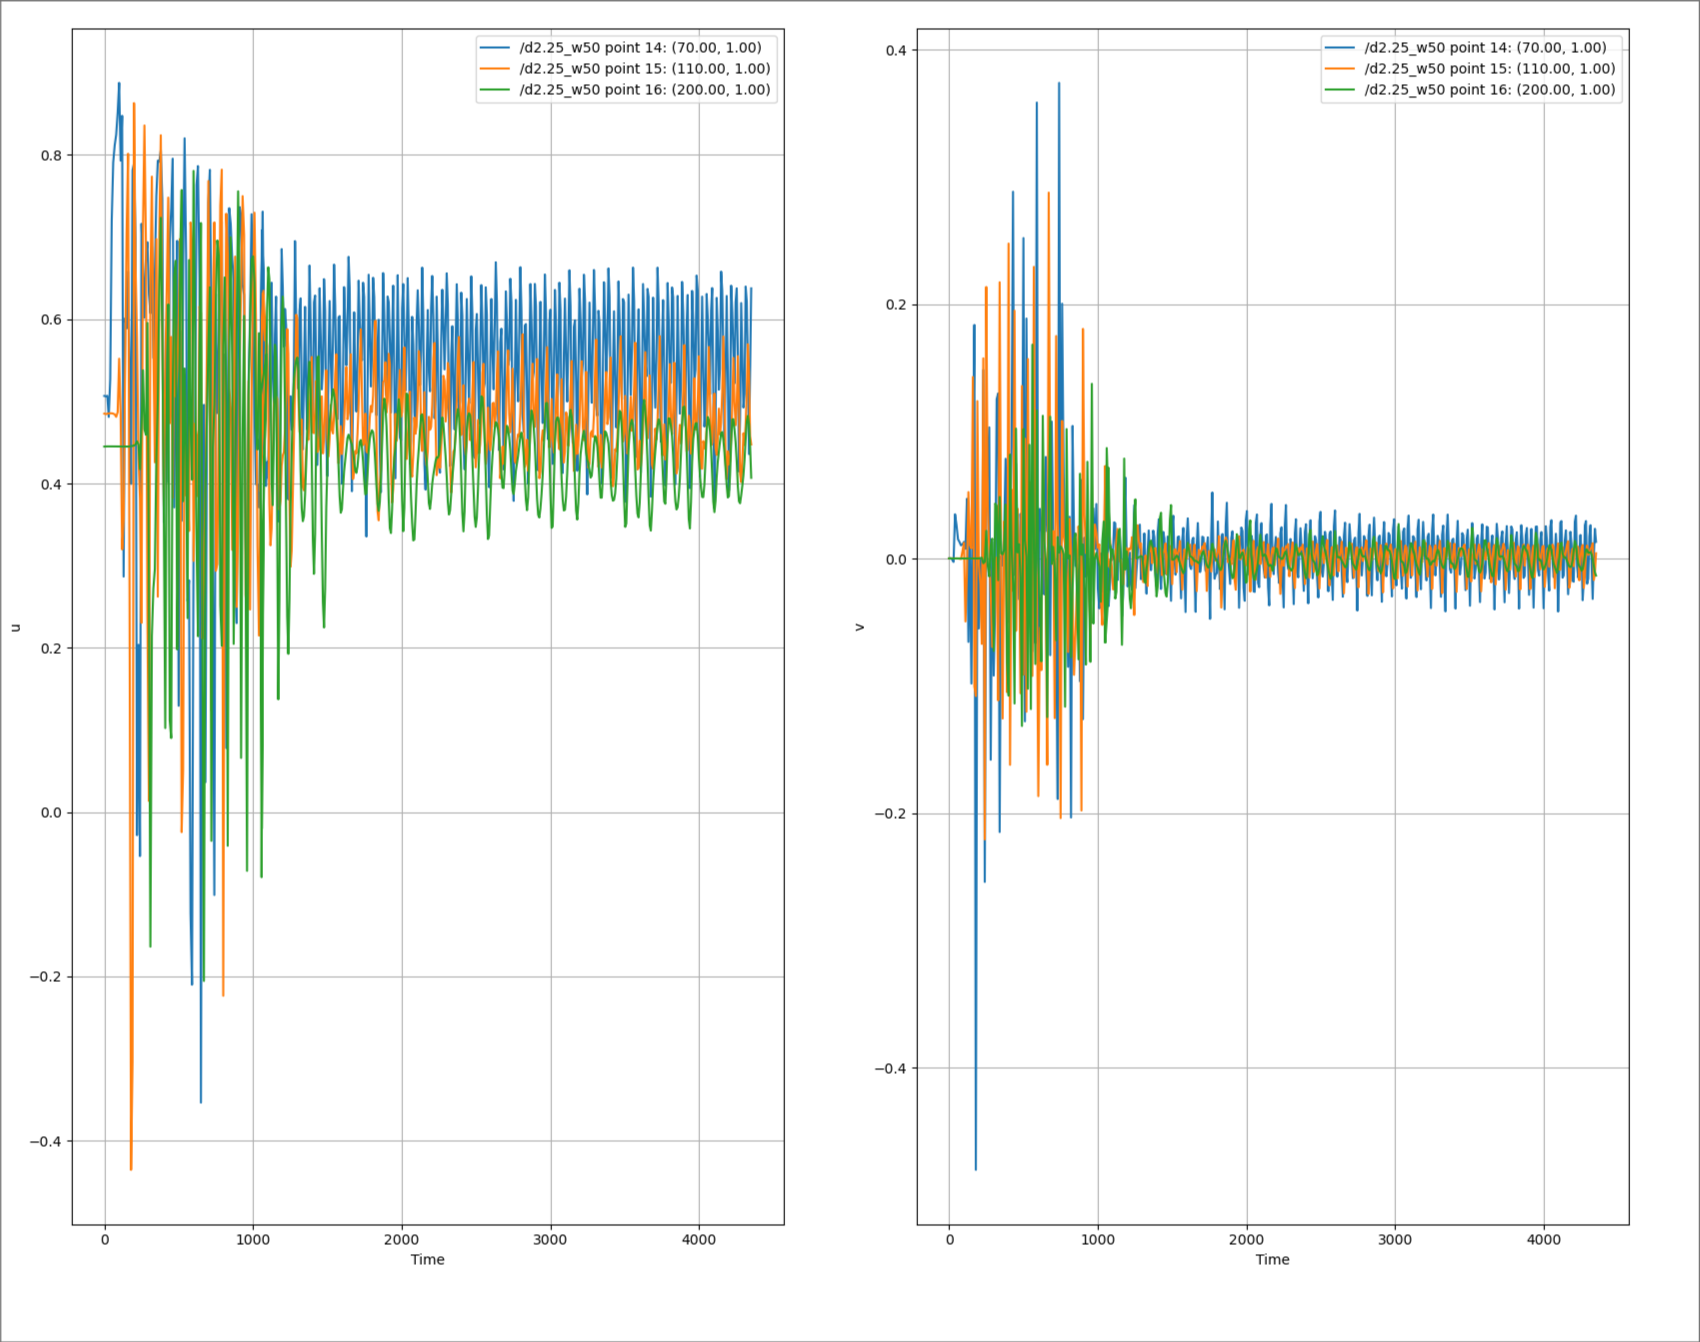
\includegraphics[width=\textwidth]{Images/d2.25_w50.png}
			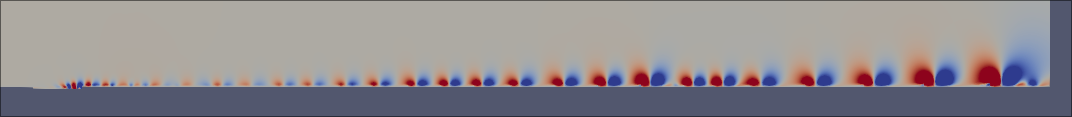
\includegraphics[width=\textwidth]{Images/d2.25_w50_dom.png}
		\end{column}
	\end{columns}
\end{frame}
\begin{frame}
	\frametitle{$d=2.25\delta^*$}
	
	\centering
	\begin{columns}[T] % [T] ensures correct vertical alignment
		\begin{column}{0.45\linewidth} % Left column
			$w=55\delta^*$

			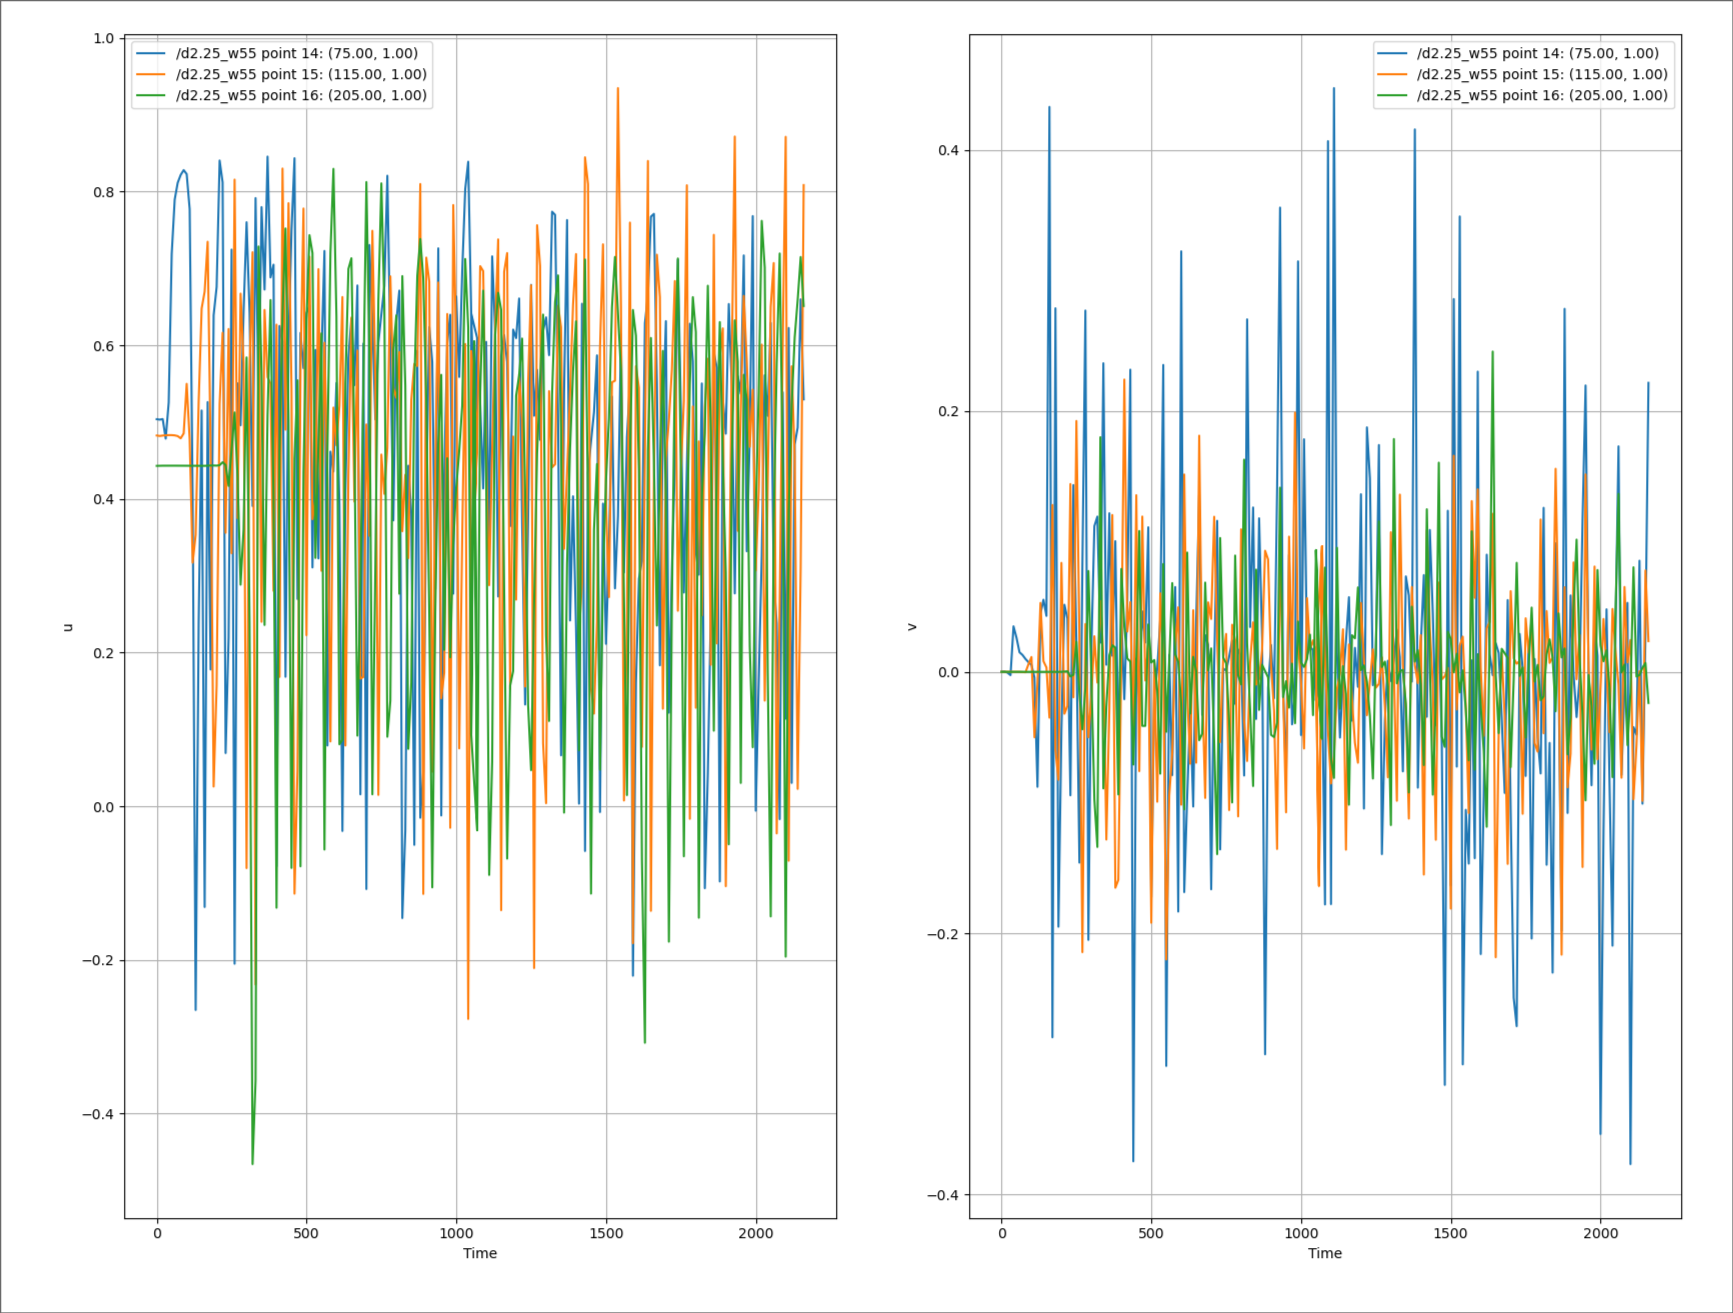
\includegraphics[width=\textwidth]{Images/d2.25_w55.png}
			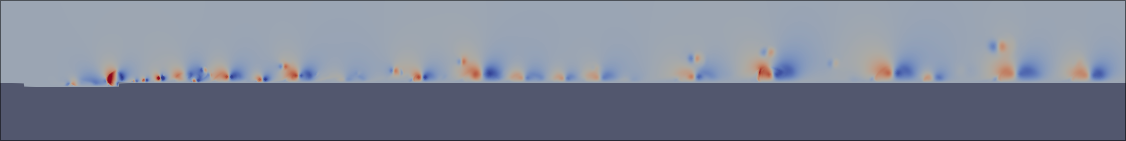
\includegraphics[width=\textwidth]{Images/d2.25_w55_dom.png}
		\end{column}
	\end{columns}
\end{frame}
\begin{frame}
	\frametitle{Absolutely unstable mode exciting TS waves}
	$d=2\delta^*$, $w=40\delta^*$

	\centering
	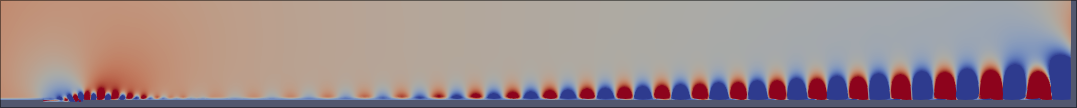
\includegraphics[width=\linewidth]{Images/d2_w40.png}
  
\end{frame}
\end{document}
